\chapter{Felhasználói dokumentáció}
Ebben a részben az alkalmazás használatáról, annak futása közben használható gyorsgombok és paraméterek beállításairól lesz szó. Ismertetem az alalmazás egyes funkcióit, továbbá a konfiguráció egyes elemeit, hogy azok milyen hatással vannak az alkalmazás működésére.

\section{Az alkalmazás használata}
Az alkalmazás Linux operációs rendszeren készült, a futtatása a konzolablakból lehetséges. A futtatáshoz a \lstinline{recognise_snooker} progam megadása szükséges, továbbá egy kötelező paraméter, amely a felismeréshez használt videófájl elérési útvonala.
\par Az egyetlen kötelező paraméteren kívül lehetséges a programnak megadni több opcionális paramétert, ezek:

\begin{itemize}
    \setlength\itemsep{-2pt}
    \item \lstinline{-start_frame=<frame>} a kezdő képkocka megadásához
    \item \lstinline{-end_frame=<frame>} a befejező képkocka megadásához
    \item \lstinline{-enable_logging} a naplófájlok készítéséhez
\end{itemize}

\par Az alkalmazás elindítása után felugrik a felismerő ablak amelyen alapértelmezetten a felismert golyók és egy adott golyó útvonala és információi szerepelnek, továbbá felugranak a finomhangoláshoz használható ablakok, ezekről a következő fejezetben lesz szó bővebben.
\par A felismerő ablak tartalmát az \textbf{A} és \textbf{D} gombok segítségével lehetséges váltani előre és hátra, a \textbf{Q} gomb segítségével ki lehet lépni az alkalmazásból, az \textbf{S} gomb segítségével pedig úgy lehet kilépni az alkalmazásból, hogy a konfigurációs fájlba a finomhangolási paraméterek mentésre kerülnek. Az \textbf{E} gomb segítségével képernyőkép készíthető, amelyet az alkalmazás a \lstinline{screenshot.png} fájlba ment el, amennyiben létezik egy fájl ezzel a névvel, az felülírásra kerül. Lehetséges még a videó megállítása, ez a \textbf{szóköz} gomb lenyomásával tehető meg. A videó megállított állapotában a \textbf{W} gomb segítségével lehet a videót előre léptetni képkockánként.
\par Amennyiben az alkalmazás indításakor megadásra került a \lstinline{-enable_logging} paraméter, a program egy napló fájlt készít a golyók helyzetéről és adatairól, ez a naplófájl a \lstinline{log.csv} fájlban kerül mentésre. A naplófájl egy részlete a \ref{tab:log_file} ábrán látható.


\begin{table}[!ht]
    \caption{A naplófálj egy részlete.}
    \label{tab:log_file}
	\footnotesize
	\centering
	\begin{tabular}{ l l l l l }
		\toprule
		FRAME & BLACK\_POSITION\_X & BLACK\_POSITION\_Y & BLACK\_DISTANCE & \dots \\
		\midrule
        0 & 120 & 212 & 0 & \dots \\
        1 & 120 & 212 & 0 & \dots \\
        2 & 120 & 212 & 0 & \dots \\
        3 & 120 & 212 & 0 & \dots \\
        4 & 121 & 211 & 1.41421 & \dots \\
        5 & 120 & 212 & 1.41421 & \dots \\
        6 & 121 & 211 & 1.41421 & \dots \\
        7 & 121 & 211 & 0 & \dots \\
        8 & 120 & 211 & 1 & \dots \\
        9 & 120 & 212 & 1 & \dots \\
        10 & 120 & 212 & 0 & \dots \\
        $\vdots$ & $\vdots$ & $\vdots$ & $\vdots$ & $\ddots$ \\
		\bottomrule
	\end{tabular}
\end{table}

A naplófájlban található értékek a jelenlegi képkockát és egyes színű golyók értékeit jelölik, ezek:

\begin{itemize}
    \setlength\itemsep{-2pt}
    \item \lstinline{FRAME} a vizsgált képkocka sorszáma
    \item \lstinline{<SZÍN>_POSITION_X} a golyó pozíció koordinátájának X eleme
    \item \lstinline{<SZÍN>_POSITION_Y} a golyó pozíció koordinátájának Y eleme
    \item \lstinline{<SZÍN>_DISTANCE} a golyó az előző képkockához képest megtett távolsága
    \item \lstinline{<SZÍN>_TOTAL_DISTANCE} a golyó teljes megtett távolságe adott képkockában
    \item \lstinline{<SZÍN>_SPEED} a golyó pillanatnyi sebessége
    \item \lstinline{<SZÍN>_AVERAGE_SPEED} a golyó átlagos sebessége az adott képpontban
\end{itemize}

\par Itt a \lstinline{<SZÍN>} egy golyó színéhez tartozó angol megfeleőt jelöl, amelyet a piros golyók esetében egy azonosító követ pl.: \lstinline{RED_2_}\dots, ez az azonosító 0 és 14 közötti étéket vehet fel.

\section{Finomhangolási paraméterek}
A finomhangolási paraméterekkel a felismerés egyes lépéseihez használt értékeket lehet módosítani valós időben. A paraméterek hangolásához néhány ablak áll rendelkezésre, amelyek csúszkákat tartalmaznak, ezekkel lehet a paramétereket módosítani. Az egyes csúszkákhoz tartozik egy azonosító, amely megadja a módosított paramétert.
\par Több módosítható paraméter létezik, ezek listája a következő:

\begin{itemize}
    \setlength\itemsep{-2pt}
    \item \lstinline{LG_<H,S,V>} és \lstinline{UG_<H,S,V>} a HSV maszkolás felső és alsó értékének beállításához (bővebben \ref{section:megv_asztal_kontur} rész)
    \item \lstinline{MIN_RAD_RATE}, \lstinline{MAX_RAD_RATE}, \lstinline{MIN_DIST_RATE}, \lstinline{PERFECTNESS} a körkeresésnél használt algoritmus paramétereinek módosításához (bővebben \ref{section:find_circles} rész)
    \item \lstinline{SHOWN_BALL_COLOR} és \lstinline{SHOWN_BALL_ID} a felismerő ablakban mutatott golyó színét és azonosítóját adják meg
\end{itemize}

\par A kilépés és mentés gyorsgomb megnyomását követően a fenti paraméterek kerülnek mentésre egy konfigurációs fájlban, ennek a neve \lstinline{config.txt}. A finomhangoláshoz használt ablak megjelenését a \ref{fig:parameter_window} ábra szemlélteti.

\begin{figure}[!ht]
    \centering
    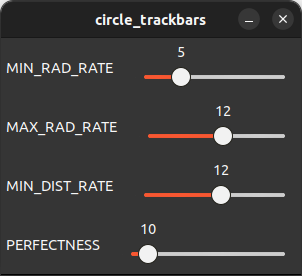
\includegraphics[width=70mm, keepaspectratio]{figures/parameter_window.png}
    \caption{Paraméterek finomhangolásához használt ablak.}
    \label{fig:parameter_window}
\end{figure}